\chapter{Microsoft Bot Framework}

The BotBuilder SDK is an open-source solution developed by Microsoft to write a chatbot in once and make it possible to connect that same chatbot to multiple channels. Examples are Skype, Slack, Facebook Messenger, etc.

\section{Business Model}

The Microsoft Bot Framework can be used in several ways. The base platform can be self-hosted on a server of choice. But to access the extra services, like spell checking, or recognizing user intents using Microsoft's LUIS (Language Understanding), an Azure subscription plan is required.

Azure is Microsoft's Cloud service that can be tailored to the customer's need. The customer can decide what modules or extra features he wants to add and calculate the price.

\begin{figure}[ht]
	\centering
	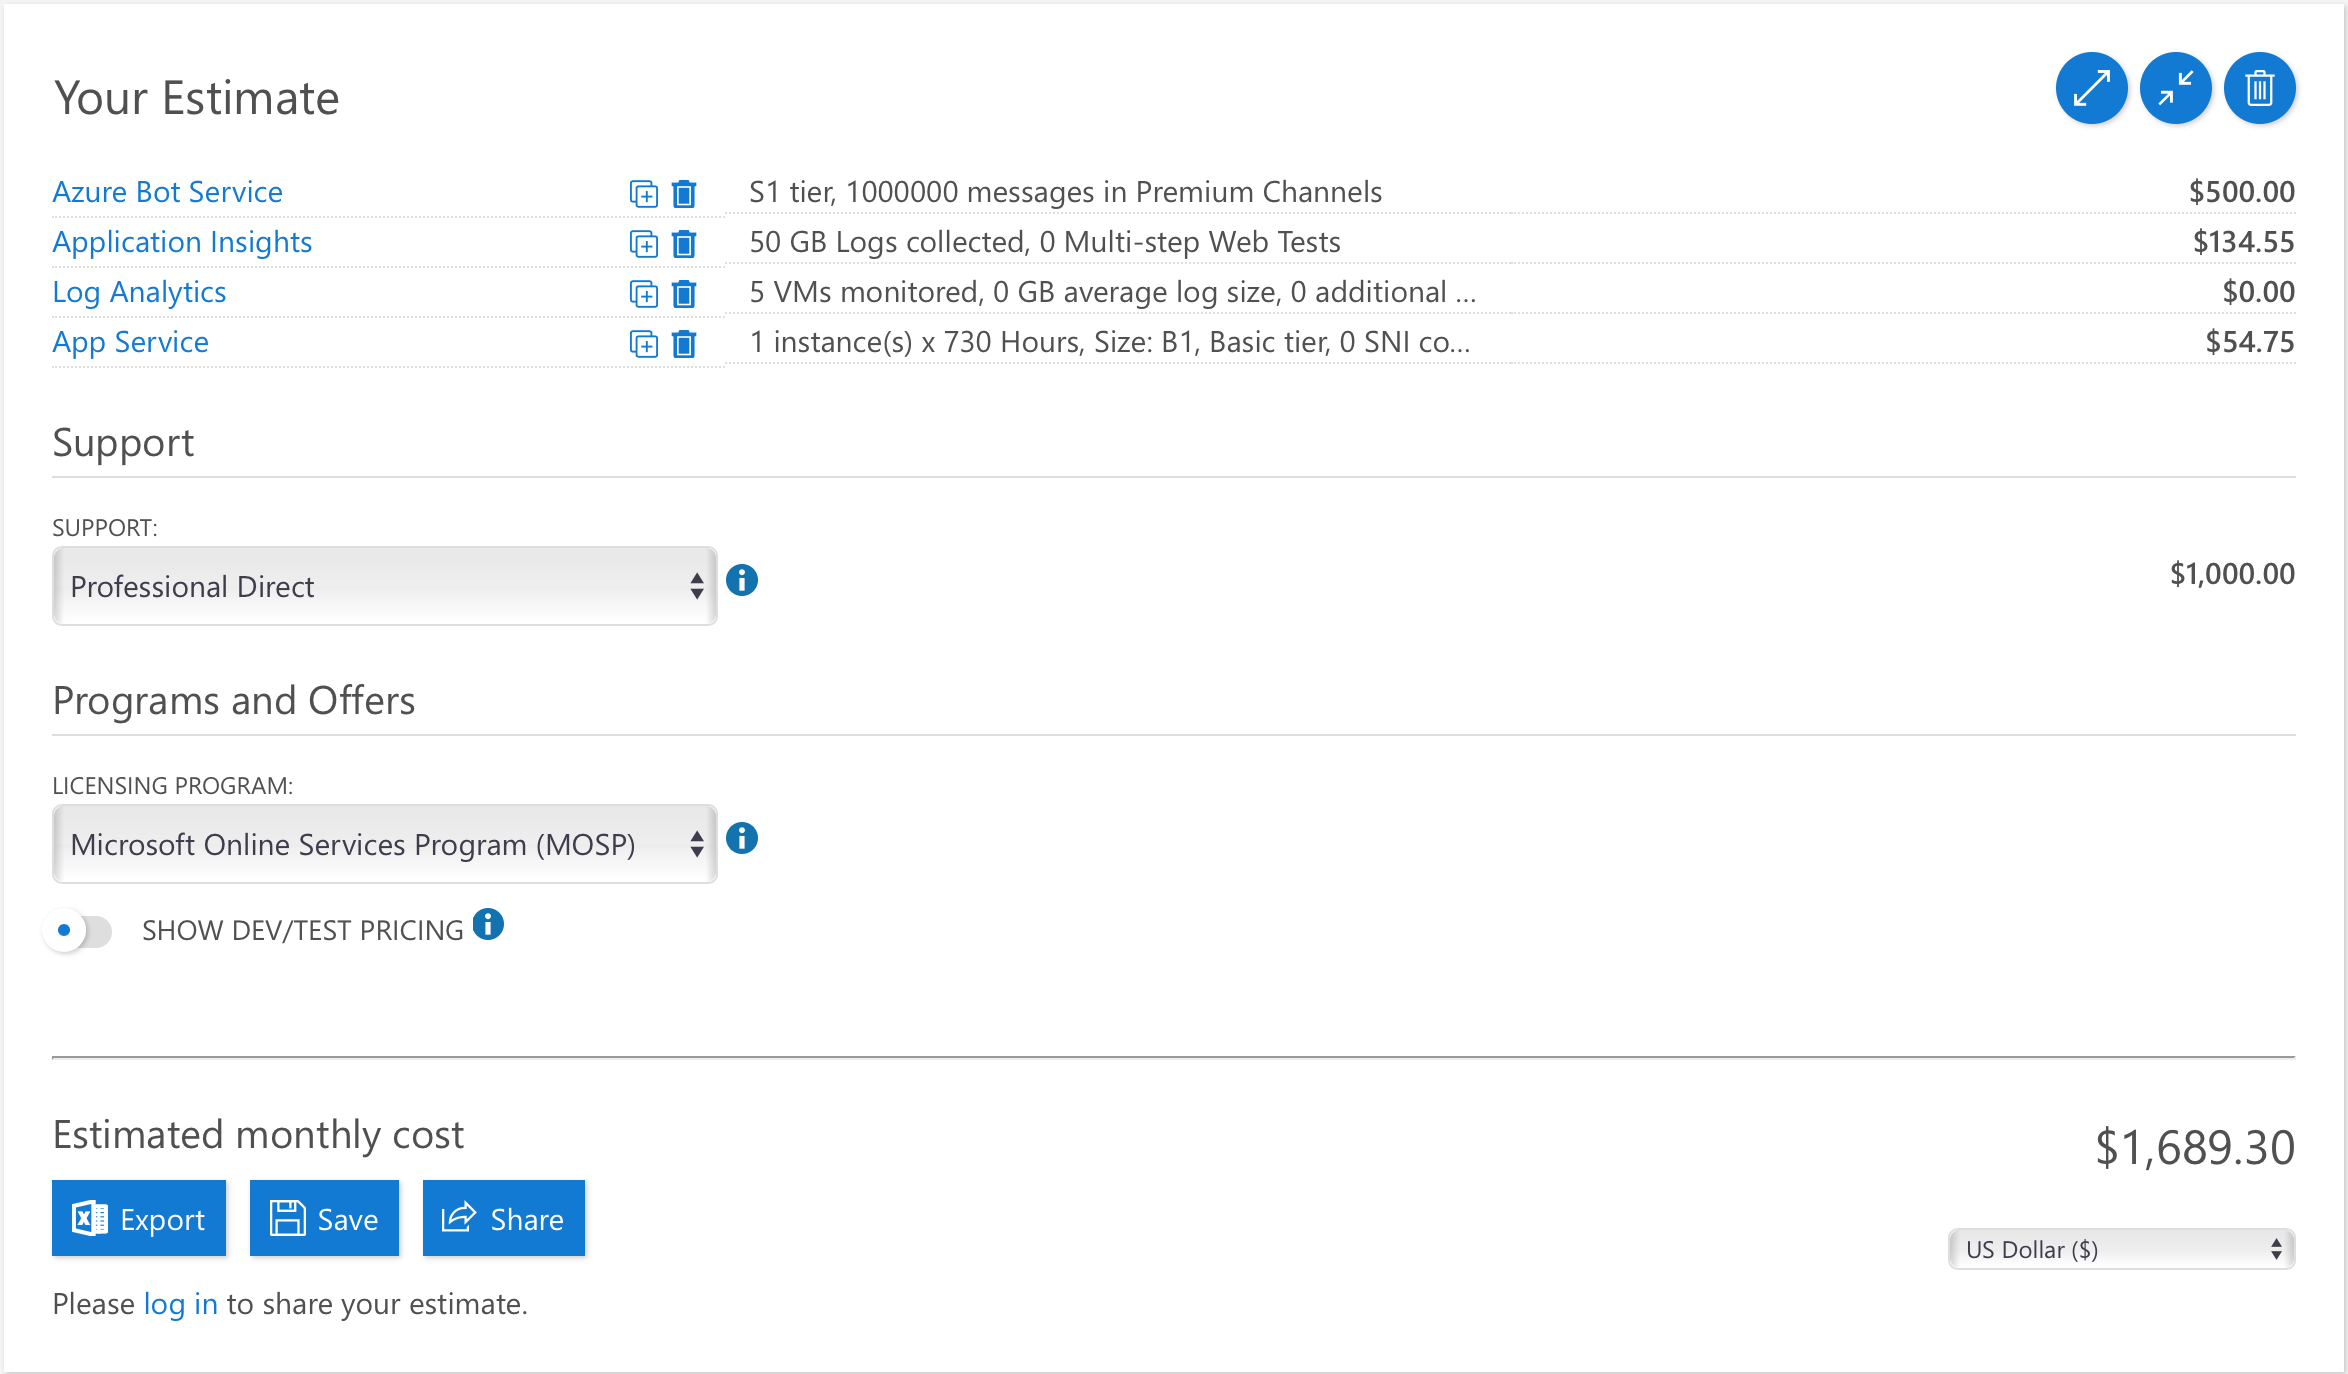
\includegraphics[width=\textwidth]{microsoft-azure-calculator-screen}\label{fig:microsoft-azure-calculator-screen}
	\caption{Microsoft's Azure Pricing Calculator~\cite{azure-pricing-calculator}}
\end{figure}

\section{Technical implementation}

Microsoft provides the bot framework for 2 languages: Node.JS and C\#. If C\# is used however, development can only be done inside of a Windows environment, or the limited online code editor.

One solution would be to use Node.JS in a code editor of choice. Preferably Visual Studio Code, Microsoft's cross-platform code editor. This way everything can be tailored and configured to the developer's needs.

\subsection{Developer environment}

Setting up a developer environment can be configured from scratch to be as complicated and complex as needed by the company or developer. Node.JS is an open-source, cross-platform JavaScript environment that can be run on a server. And in the end that's what a chatbot is, a sever API that responds to requests (messages or events from the user).

It's important to note that JavaScript or also called \Gls{ECMAScript} is a language that is advancing very quickly and Node.JS cannot keep up with all the newest yearly features. And all of the documentation involving the Bot Framework is written in \Gls{ES5}. However it's still possible to use all of the newest features of ECMAScript if you compile your code down the ES5.

The documentation on setting up an environment like this is very limited. Microsoft does not provide any instructions or boilerplates on how to set up an efficient environment. This allows for more freedom but increases the learning curve for a developer who wants to start coding a bot using newer ECMAScript features or the option to hot reload his code.

\subsubsection{Project structure}

Structuring the project is straight forward. Just like most production JavaScript projects there is a source folder containing all of the actual source code. Developers can decide to divide the test files into a separate folder but generally it's recommended to keep the test files close to the source file they reference.

The node\_modules folder is a dependency folder, this contains any dependencies needed to build the project. There are two types of dependencies: Firstly there are developer-dependencies, these are dependencies needed to build the project and participate in development. An example is eslint, these are a set of specific language rules configured for the project to follow. There are also regular dependencies, these are external libraries the project might use to do calculations, or wrappers for certain technologies. The Microsoft Bot Framework works using their botbuilder \Gls{SDK} as a dependency.

Next up are the config files, these are the workhorses of the developer's environment. There are 2 separate configuration files for the developers to build and test the bot as for the production server to build a functional output file. Webpack is a very powerful, well documented build tool and allows for easy customization. It is commonly used for front-end development but after some tweaking it can be used for Node.JS development as well. The development config starts a server that hot-reloads any changes made to the source files. This way it's easy for the developer to seamlessly check his changes instead of manually recompiling and restarting the server. The production config is very straightforward and simply compiles a minified and optimized output file into the build folder.

Further more there is support for environment variables using the dotenv dependency. This file is not versioned to git and will contain any API keys used in the project.

\begin{figure}[ht]
	\centering
	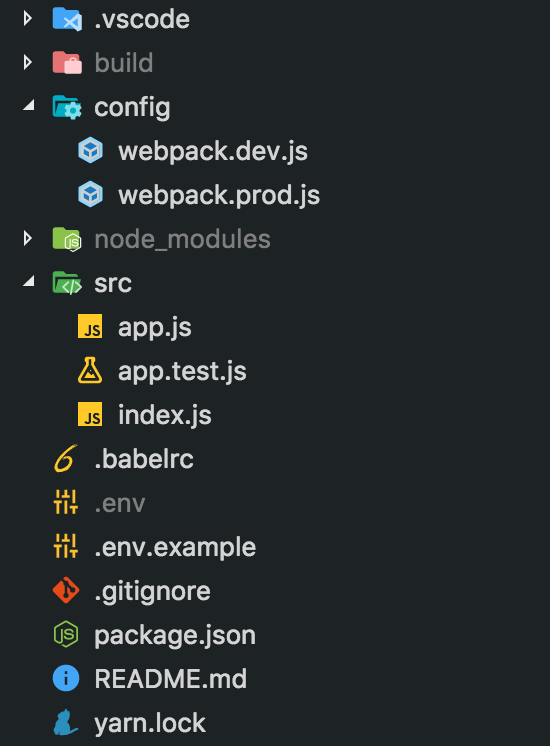
\includegraphics[width=0.33\textwidth]{projectstructure}\label{fig:projectstructure}
	\caption{Project structure}
\end{figure}

\subsection{Testing}

The bot can be tested locally or remotely on any platform using Microsoft's own Bot Emulator~\cite{microsoft-bot-emulator}, which is also open-source. This provides the developer with a live testing interface and information about everything the bot receives, including requests and the data that comes with them.

Speech Recognition is also supported for speech enabled bots. Sending system activities is another useful feature because it allows the developer to emulate user events like for example a user joining the conversation. Lastly, payment processing is supported as well to emulate a transaction.

\begin{figure}[!hb]
	\centering
	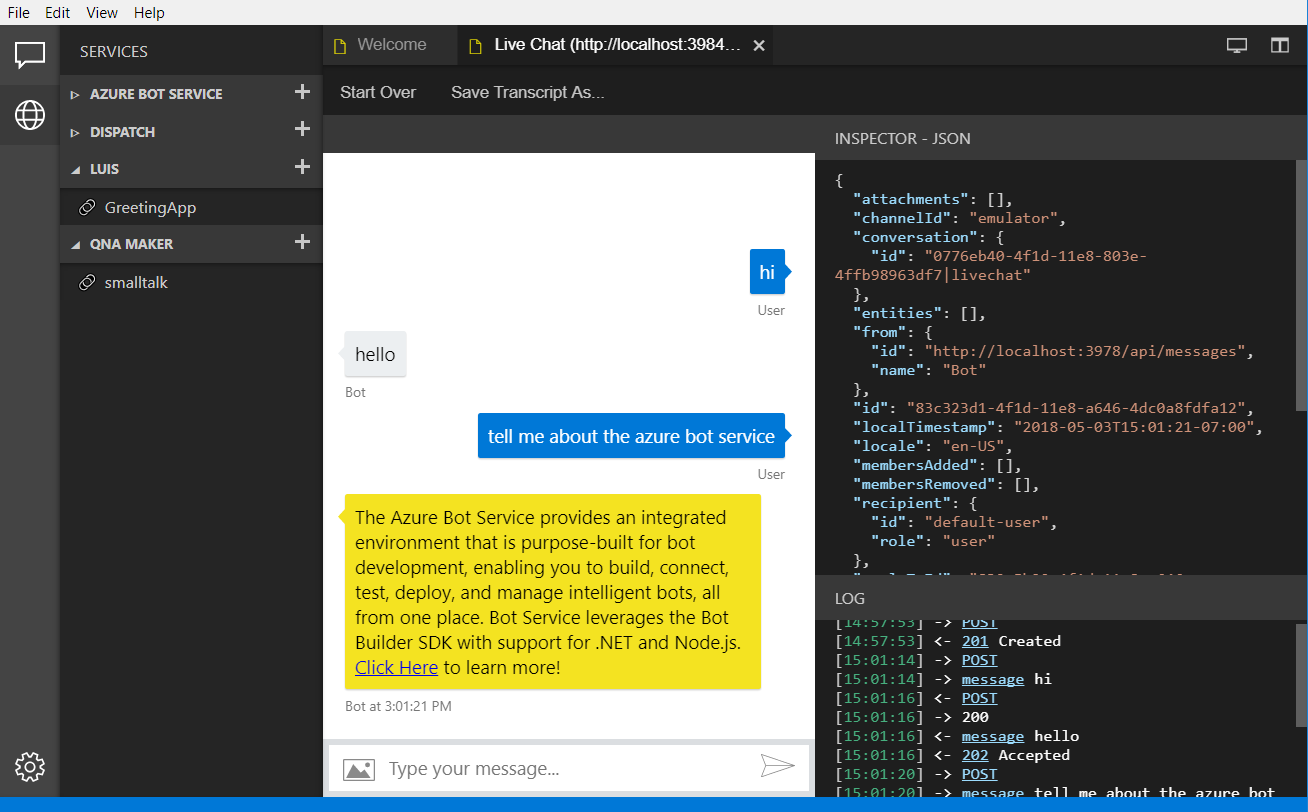
\includegraphics[width=0.85\textwidth]{microsoft-bot-emulator}\label{fig:microsoft-bot-emulator}
	\caption{Microsoft's Bot Emulator~\cite{microsoft-bot-emulator}}
\end{figure}

\section{Building the bot}

\subsection{Initialization}

Initializing the bot is straightforward, the official documentation recommends restify as the server. During initialization it's also possible to define a default message the bot will always use as a reply if no other reply options match.

\begin{lstlisting}[language=JavaScript,caption=Initialization of the chatbot,label=listing:botframework-init]
import restify from 'restify';
import * as builder from 'botbuilder';

// Setup Restify Server
const server = restify.createServer();
server.listen(process.env.port || process.env.PORT || 3978, () => {
	console.log('%s listening to %s', server.name, server.url); 
});

// Create chat connector for communicating with the Bot Framework Service
const connector = new builder.ChatConnector({
		appId: process.env.MicrosoftAppId,
		appPassword: process.env.MicrosoftAppPassword
});

// Listen for messages from users 
server.post('/api/messages', connector.listen());

const bot = new builder.UniversalBot(connector, (session) => {
	session.send(
		"Sorry, I didn't get that. Type 'help' if you need assistance or try a different sentence.",
		session.message.text,
	);
}).set('storage', inMemoryStorage);
\end{lstlisting}

To make the bot start the conversation certain events can be used. In this case a `conversationUpdate' event will be used to trigger the root dialog.

\begin{lstlisting}[language=JavaScript,caption=Initial message,label=listing:botframework-init-message]
bot.on('conversationUpdate', (message) => {
	if (message.membersAdded) {
		message.membersAdded.forEach((identity) => {
			if (identity.id === message.address.bot.id) {
				bot.beginDialog(message.address, '/welcome');
			}
		});
	}
});
\end{lstlisting}

\newpage

\subsection{Event types}
\begin{itemize}
	\item message
	\item conversationUpdate
	\item contactRelationUpdate
	\item typing
	\item ping
	\item deleteUserData
	\item endOfConversation
	\item event
	\item invoke
	\item messageReaction
\end{itemize}

The previous listing lists all of the available events during a conversation. A message event simply represents any communication between bot and user. The conversationUpdate event is triggered when any members are added/removed from the conversation, including the bot. Or when conversation metadata has changed. The contactRelationUpdate event indicates that the bot was added or removed to a user's contact list.

Most of these events can be triggered using the bot emulator or in code and sending it to the bot. This last one is useful for unit testing.

\begin{lstlisting}[language=JavaScript,caption=Sending a mock event to the bot,label=listing:botframework-mock-event]
const event = {
	address: { bot: { id: '0' }, user: { id: 0 } },
	agent: 'botbuilder',
	source: 'facebook',
	sourceEvent: '',
	type: 'conversationUpdate',
	membersAdded: [{ id: '0', isGroup: false, name: 'test' }],
	user: { id: '0', isGroup: false, name: 'test' },
};

connector.processEvent(event);
\end{lstlisting}

\section{Constructing a conversational flow}

One of the key concepts in the Bot Builder SKD are dialogs. Dialogs help the developer manage the conversational logic and is a fundamental part of developing a chatbot in the bot framework.

A dialog can be compared to a function. It can perform a specific task and be called at any point in time. Dialogs can also contain other dialogs to advance and branch off a conversation.

A waterfall is an example of a dialog that guides the user through a set amount of steps or tasks. A great example of this is ordering food. First the user will be asked for drinks, followed up by the amount, again followed up by what starters the user wants and so on. There is a clear structure the bot goes through, hence the name Waterfall.

A waterfall is defined by creating an array of consecutive functions or waterfall steps inside of a dialog.

\subsection{Prompts}

To help the bot wait for a reply Microsoft provides developers with so called `Prompts'. These already contain some extra functionality to validate the user's reply. A prompt should be used whenever the bot expects a reply from the user.

\subsubsection{Prompt types}

\begin{itemize}
	\item text
	\item confirm
	\item number
	\item time
	\item choice
	\item attachment
\end{itemize}

When used inside of a waterfall dialog, the reply of the user will be passed to to next step using the `results' object. Another method called `next' can be used from the arguments to skip to the next step of the waterfall.

\begin{lstlisting}[language=JavaScript,caption=2-step waterfall using a prompt,label=listing:waterfall-and-prompt]
bot.dialog('orderButtonClick', [
	(session) => {
		builder.Prompts.choice(session, 'Thirsty? Want to order any drinks?', 'Yes|No drinks', {
			listStyle: builder.ListStyle.button,
		});
	},
	(session, results, next) => {
		if (results.response.entity === 'Yes') {
			session.beginDialog('orderDrink');
		} else {
			next();
		}
	},
]);
\end{lstlisting}

\subsection{User actions}

There's multiple ways to handle user input other than prompts. Another way of doing this is using actions.

\subsubsection{Triggeraction}

The most common action is a `triggerAction'. This can be connected to a dialog to invoke it whenever the user inputs a matched term. Whenever this is triggered, the dialog stack is cleared and the invoked dialog will be the new first dialog on the stack.

This behavior isn't always desired when the conversation needs to be temporarily redirected and resumed later on. That's where the `onSelectAction' option comes in, to add the matched dialog to the existing stack.

\subsubsection{BeginActionDialog}

A specific dialog can also be attached to a dialog using the `beginActionDialog' function. This can be useful to send the user to a contextual action. An example of this is when the user asks for specific help in a dialog context.

\subsubsection{CustomAction}

Unlike all the other actions, a customAction does not have any default action defined. It's up to the developer to define what it should do. The main benefit of using these is providing quick answers to a user without manipulating the dialog stack at all.

Further more a customAction does not bind to a dialog, instead it binds to the bot itself.

\subsubsection{ReloadAction}

The reloadAction is pretty self-explanatory. Binding this to a dialog means it will restart the dialog whenever the action is invoked. It's also possible to pass arguments to this action for the dialog to receive.

\subsubsection{CancelAction}

This action cancels the dialog it is bound to when triggered. The parent dialog will also receive an indication the child dialog was canceled.

\subsubsection{EndConversationAction}

Similar to the cancelAction action, the endConversation action will end the entire conversation when triggered. This clears the entire dialog stack and persisted state data.

\subsubsection{Important to note}

Important to note is the fact that some of these actions are quite interruptive to the conversation's flow. To make sure the user really wants to clear the entire dialog stack and start over, a confirm prompt can also be added to these actions.